\documentclass[aps,11pt,twoside,nofootinbib,tightenlines,superscriptaddress,preprintnumbers]{revtex4}

%%% macro %%%

\usepackage{amsfonts,amssymb}
\usepackage{graphicx}
\usepackage{epic}
%\usepackage{biblatex} this cause bug
\usepackage{soul}
\usepackage{amsmath}
\bibliography{ref.bib}

%%%%%%%%%%%%%%%%%%%%%%%%%%%%%%%%%%%%%%%%%%%%%%%%%%%%%%%%%%%%%%%%%%%%%%%%%%%%%%%
% Definitions

\newcommand{\<}{\langle}
\renewcommand{\>}{\rangle}

\newcommand{\be}{\begin{equation}}
\newcommand{\ee}{\end{equation}}
\newcommand{\bea}{\begin{eqnarray}}
\newcommand{\eea}{\end{eqnarray}}

\newcommand{\cond}[1]{\left\{\begin{array}{l@{~~~}l}#1\end{array}\right.}
\newcommand{\qph}[1]{quant-ph/#1}

\newcommand{\BPP}{{\mathrm{BPP}}}
\newcommand{\BQP}{{\mathrm{BQP}}}
\newcommand{\ent}{{\textsc{entrance}}}
\newcommand{\exit}{{\textsc{exit}}}
\renewcommand{\root}{{\textsc{root}}}

\renewcommand{\d}{{\mathrm{d}}}
\newcommand{\sech}{\mathop{\mathrm{sech}}\nolimits}
\newcommand{\Ai}{\mathop{\mathrm{Ai}}\nolimits}
\newcommand{\poly}{\mathop{\mathrm{poly}}\nolimits}
\newcommand{\col}{\mathop{\mathrm{col}}\nolimits}

\newcommand\symProb{\mathop{\mathrm{Pr}}\displaylimits}
\newcommand\symExpec{\mathop{\mathrm{E}}\displaylimits}
\def\prob#1#2{\symProb_{#1}\left[ #2 \right]}
\def\expec#1#2{\symExpec_{#1}\left[ #2 \right]}

\newtheorem{theorem}{Theorem}
\newtheorem{lemma}[theorem]{Lemma}
\newtheorem{game}{Game}

\newcommand{\qed}{\rule{7pt}{7pt}}
\newenvironment{proof}
  {\trivlist\item\noindent{\bf Proof}~}
  {\qed\endtrivlist}
  
\newenvironment{proof sketch}
{\trivlist\item\noindent{\bf Proof sketch}~}
{\qed\endtrivlist}


%%%%%%%%%%%%%%%%%%%%%%%%%%%%%%%%%%%%%%%%%%%%%%%%%%%%%%%%%%%%%%%%%%%%%%%%%%%%%%%

%%% Info %%%

\title{Exponential algorithmic speedup by quantum walk}

\begin{document}

\title{A Survey: Exponential algorithmic speedup by quantum walk}

\author{Yan-Tong Lin}
\email[]{0312fs3@gmail.com}
\affiliation{Department of Computer Science,
             National Chiao Tung University,
             Hsinchu, Taiwan}

\date[]{11 Jan 2021}

\preprint{Quantum Computation and Quantum Information Final Report}

%%%%%%%%%%%%%%%%%%%%%%%%%%%%%%%%%%%%%%%%%%%%%%%%%%%%%%%%%%%%%%%%%%%%%%%%%%%%%%%
% Abstract

\begin{abstract}
The authors construct an oracular problem (based on a random graph) that provide the first exponential quantum-classical algorithmic separation based on quantum walks. They show how to implement the continuous time quantum walk, provide physical intuition, and prove the time upper bound. Finally, the main contribution of the paper is the proof that no classical algorithm can solve the problem with high probability in subexponential time. In this survey, I will try to present the core values of the 24-page paper and sketch the proofs so that they are easier to understand.
\end{abstract}

\maketitle

%%%%%%%%%%%%%%%%%%%%%%%%%%%%%%%%%%%%%%%%%%%%%%%%%%%%%%%%%%%%%%%%%%%%%%%%%%%%%%%

\section{Preliminaries} \label{sec:pre}
To understand this paper, one is expected to have some basic knowledge in the following fields.
\begin{itemize}
    \item linear algebra
    \item calculus
    \item complexity theory
    \item graph theory
    \item quantum postulates
\end{itemize}{}

\section{Introduction and Problem Definition} \label{sec:intro}
Simon's algorithm \cite{Sim94} provides an exponential separation between $\BQP^{A}$ and $\BPP^{A}$ with an oracle $A$ and it uses quantum Fourier transformation as its backbone. A previous work \cite{FG98} shows an exponential gap between random walk and its quantum counterpart --- quantum walk with graph $G_n$ (Figure \ref{fig:graph}). This paper, at that time, was the first to provide exponential separation between $\BQP^{A}$ and $\BPP^{A}$ with an oracle $A$ corresponding to graph $G^{\prime}_n$ (Figure \ref{fig:graphprime}), using quantum walk. \footnote{Please note that the relation of complexity classes relative to oracles provides intuitions and insights to the relation of original classes, but it cannot be used to show the relation itself.\cite{MITACT16}}

We define the problem as follow --- given an oracle for the graph and the name of the $\ent$, find the name of the $\exit$. The construction of the graph is shown by examples in Figure \ref{fig:graph} and Figure \ref{fig:graphprime}. Despite that classical random walk requires steps exponential in $n$ to find the $\exit$ with high probability, one can easily construct a classical algorithm to solve the traversal problem using the fact that nodes in the middle are with degree $2$.

For the rest of this survey, I will introduce quantum walk and show its efficiency in Section \ref{sec:algorithm} and demonstrate the classical lower bound in Section \ref{sec:algorithm}. Some details of the proofs will be skipped and you may find them in the original paper \cite{EXP03}.

\begin{figure}
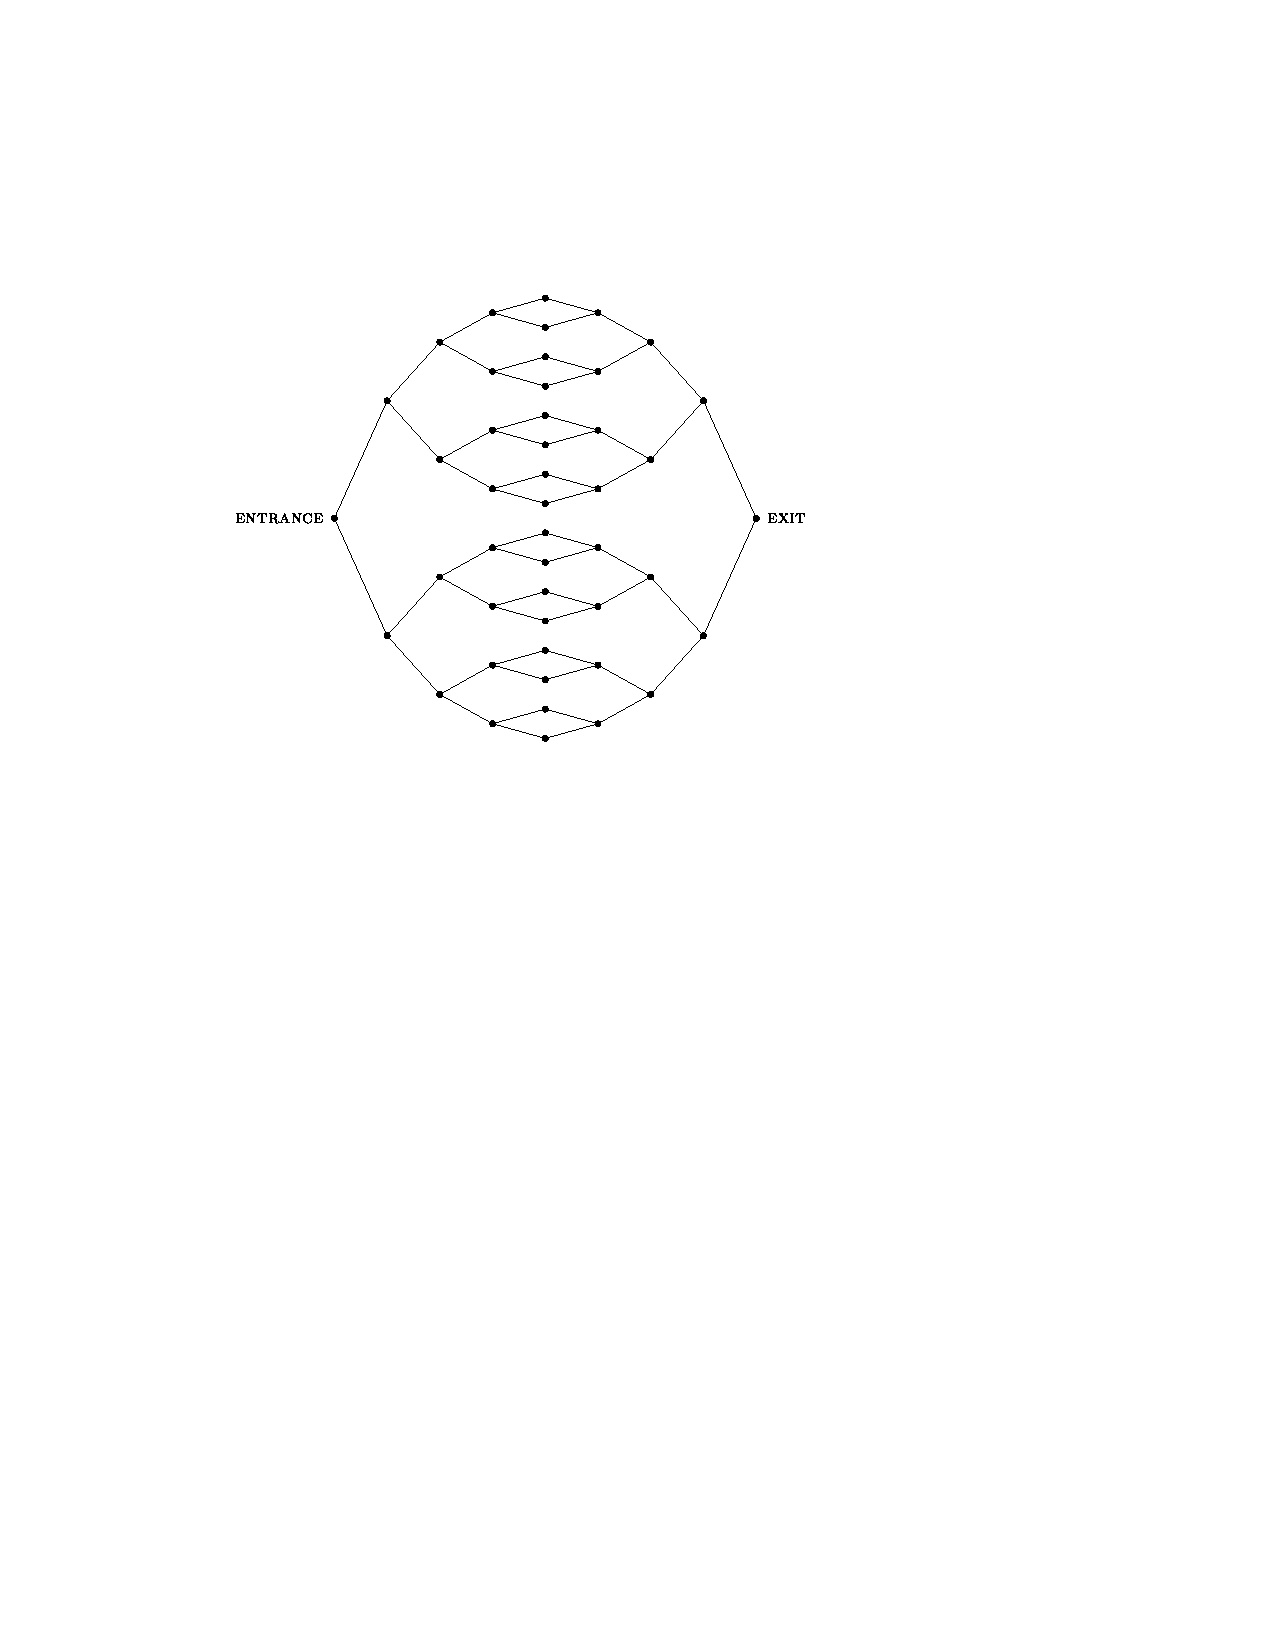
\includegraphics[width=280pt]{basicgraph4}
\caption{The graph $G_4$.}
\label{fig:graph}
\end{figure}

\begin{figure}
\includegraphics[width=284pt]{graph4}
\caption{A typical graph $G^{\prime}_4$.}
\label{fig:graphprime}
\end{figure}

%%%%%%%%%%%%%%%%%%%%%%%%%%%%%%%%%%%%%%%%%%%%%%%%%%%%%%%%%%%%%%%%%%%%%%%%%%%%%%%
\section{Quantum algorithm}\label{sec:algorithm}

%%%%%%%%%%%%%%%%%%%%%%%%%%%%%%%%%%%%%%%%%%%%%%%%%%%%%%%%%%%%%%%%%%%%%%%%%%%%%%%
\subsection{Quantum walk}\label{subsec:qwalk}

\subsubsection{Classical random walk}

To know what is a quantum walk, one may better be familiar with its classical counter part.

In a continuous time classical random walk (which is also known as a Markov process), there is a fixed probability per unit time $\gamma$ of moving to an adjacent vertex.  In other words, from any
vertex, the probability of jumping to any connected vertex in a time $\epsilon$ is $\gamma \epsilon$ (in the limit $\epsilon \to 0$).  If the graph has $N$ vertices, the random walk can be described by the $N \times N$ infinitesimal generator matrix $K$ defined by
\be
  K_{aa'} = \cond{ 
      \gamma       & a \ne a', \ aa' \in G \\
      0            & a \ne a', \ aa' \notin G \\
      -d(a) \gamma & a=a' \,.}
\ee
If $p_a(t)$ is the probability of being at vertex $a$ at time $t$, then
\be
  {\d p_a(t) \over \d t} = \sum_{a'} K_{aa'} \, p_{a'}(t)
\,.
\label{eq:diffeq}
\ee
Note that because the columns of $K$ sum to zero, an initially normalized
distribution remains normalized, i.e., $\sum_a p_a(t) = 1$ for all $t$.

\subsubsection{Quantum Analog}

Now consider quantum evolution in an $N$-dimensional Hilbert space spanned
by states $|1\>, |2\>, \ldots, |N\>$ corresponding to the vertices of $G$.
If the Hamiltonian is $H$, then the dynamics of the system are determined
by the Schr\"odinger equation,
\be
  i {{\mathrm d} \over {\mathrm d}t} \<a|\psi(t)\> 
    = \sum_{a'} \<a|H|a'\> \<a'|\psi(t)\>
\,.
\label{eq:schrodinger}
\ee

Its natural to consider a quantum evolution corresponding to a Hamiltonian equals to s the adjacency matrix of the graph times $\gamma$.
\be
  \<a|H|a'\> = \cond{ \gamma & a \ne a', \ aa' \in G \\
                      0      & \textrm{otherwise.} }
\label{eq:graphham}
\ee
Because $H$ is Hermitian, probability is conserved, i.e., $\sum_a
|\<a|\psi(t)\>|^2=1$ for all $t$.

This will be the quantum walk we uses in this paper. \footnote{Please note that there can be many realizations of "quantum walk", as long as they make sense.} Now our goal is to simulate the unitary evolution $e^{-i H t}$ with $H$ given by (\ref{eq:graphham}).

%%%%%%%%%%%%%%%%%%%%%%%%%%%%%%%%%%%%%%%%%%%%%%%%%%%%%%%%%%%%%%%%%%%%%%%%%%%%%%%
\subsection{Implementing the quantum walk}\label{subsec:implement}

\subsubsection{The oracle}

To show how to implement the quantum walk, we start by defining oracles corresponding to graphs rigorously.

To make an oracle, we require that the graph comes with additional structures so that the oracle is unitary. \footnote{It remains an open problem to construct efficient oracles for general graphs} In this paper we take consistent coloring --- an edge coloring that no vertex is incident with two edges of the same color --- as the additional structure. The coloring will be given in the Section \ref{sec:lowerbound} and we will show that the coloring can be made up by classical algorithms so it cannot provide more information to solve the problem. 

Assuming a consistent $k$-coloring of the graph is given. Let $n=\lceil \log N \rceil$ so it takes $n$ bits to list the vertices of the graph $G$.  In the classical setting, the black box takes two inputs, a name $a$ given as a $2n$-bit \footnote{we use $2n$ so that there is exponentially more names than vertices} string and a color $c$.  If the input name $a$ corresponds to a vertex that is incident with an edge of color $c$, then the output is the name of the vertex joined by that edge, otherwise the output is the special bit string $11\ldots1$, which is not the name of any
vertex. For shorthand, we write $v_c(a)=a'$, where $a$ is the input name, $c$ is the color, and $a'$ is the output name. Note that $v_c(v_c(a))=a$ for $v_c(a) \ne 11\ldots1$.

The unitary quantum oracle corresponding to this classical black box is
described as follows.  Let $a,b$ be $2n$-bit strings and let $c$ be a
color.  Then the action of the quantum black box $U$ associated with the graph $G$ is
\be
  U |a,b,c\> = |a,b \oplus v_c(a),c\>
\label{eq:graphoracle}
\ee
Since we will never need to query $U$ with superposition of colors, it is sufficient to omit the color register and assume that we have access to the $k$ unitaries
\be
  U_c|a,b\> = |a,b \oplus v_c(a)\>
\,,
\ee
one for each of the $k$ possible colors. In fact, since we want to check whether $v_c(a)=11\ldots1$, it is also straightforward to extend the Hilbert space by a single qubit and perform each of the $k$ transformations
\be
  V_c|a,b,r\> = |a,b \oplus v_c(a),r \oplus f_c(a)\>
\,,
\label{eq:simpleoracle}
\ee
where
\be
  f_c(a) = \cond{
      0 & v_c(a) \ne 11\ldots1 \\
      1 & v_c(a) = 11\ldots1\,.}
\ee

The Hilbert space that $V_c$ acts on in (\ref{eq:simpleoracle}) has dimension $2^{4n+1}$, which is much larger than the number of vertices in the graph.  We want the quantum evolution $e^{-i H t}$ to take place in an $N$-dimensional subspace. To this end, we will show how to implement the
quantum walk given the oracles $V_c$ in the sense that we will construct a Hamiltonian $H$ satisfying
\be
  H |a, 0, 0\> = \sum_{c:\, v_c(a) \in G} |v_c(a),0,0\>
\,.
\label{eq:ham}
\ee
This means that if we start our evolution in the subspace of states of the
form $|a,0,0\>$ where $a \in G$, then we will remain in this
$N$-dimensional subspace.

\subsubsection{Tools for simulating Hamiltonians}

In general, it is not easy to answer the question of whether a particular Hamiltonian can be simulated efficiently. However, there are some useful standard tools for
simulating Hamiltonians.  The following is a list of five such tools, four
of which will be used in our construction. \cite{NC00}

\begin{enumerate}
\item {\em Local terms.}
\item {\em Linear combination.}  
\item {\em Commutation.} 
\item {\em Unitary conjugation.}
\item {\em Tensor product.} 
\end{enumerate}

\subsubsection{$T$ operator for swapping or deleting information}

We want to turn $V_c$ into $H$, so we define a Hermitian $T$ as follow,
\bea
  T |a, b, 0\> &=& |b, a, 0\> \\
  T |a, b, 1\> &=& 0
\,.
\eea

The operator $T$ may be written as
\be
  T = \left( \bigotimes_{l=1}^{2n} S^{(l,2n+l)} \right) \otimes |0\>\<0|
\label{eq:swap}
\ee
where the superscript indicates which two qubits $S$ acts on, and the
projector onto $|0\>$ acts on the third register.  Here $S$ is a Hermitian
operator on two qubits satisfying $S |z_1 z_2\> = |z_2 z_1\>$.

Since the eigenvalues of $S$ are $\pm1$, the eigenvalues of $T$ are $0,\pm1$, and
they are easy to compute. Thus $e^{-i T t}$ can be simulated with the
circuit shown in Figure~\ref{fig:simT}.  In this figure, $W$ denotes a
two-qubit unitary operator that diagonalizes $S$.  The unique eigenvector
of $S$ with eigenvalue $-1$ is ${1 \over \sqrt2}(|01\>-|10\>)$, so we take
\bea
  W |00\> &=& |00\> \\
  W {\textstyle{1 \over \sqrt2}}(|01\> + |10\>) &=& |01\> \\
  W {\textstyle{1 \over \sqrt2}}(|01\> - |10\>) &=& |10\> \\
  W |11\> &=& |11\>
\,.
\eea
Applying $W^{\otimes 2n}$ diagonalizes $T$, and the Toffoli gates compute
the argument of the eigenvalue in an ancilla register initially prepared
in the state $|0\>$. After that, we apply the appropriate phase shift ($Z$ or $I$) by parity of the ancillary bit indicating the eigenvalue. Finally, we uncompute the ancillary bit and return to the original basis.

\begin{figure}
\setlength{\unitlength}{2pt}
\begin{picture}(180,105)
\put(10,5){\line(1,0){78}}
\put(102,5){\line(1,0){78}}
\put(10,15){\line(1,0){84}}
\put(96,15){\line(1,0){84}}
\put(10,25){\line(1,0){10}}
\put(40,25){\line(1,0){39}}
\put(81,25){\line(1,0){28}}
\put(111,25){\line(1,0){39}}
\put(170,25){\line(1,0){10}}
\put(10,35){\line(1,0){10}}
\put(40,35){\line(1,0){110}}
\put(170,35){\line(1,0){10}}
\put(10,65){\line(1,0){10}}
\put(40,65){\line(1,0){19}}
\put(61,65){\line(1,0){68}}
\put(131,65){\line(1,0){19}}
\put(170,65){\line(1,0){10}}
\put(10,75){\line(1,0){10}}
\put(40,75){\line(1,0){110}}
\put(170,75){\line(1,0){10}}
\put(10,90){\line(1,0){10}}
\put(40,90){\line(1,0){9}}
\put(51,90){\line(1,0){88}}
\put(141,90){\line(1,0){9}}
\put(170,90){\line(1,0){10}}
\put(10,100){\line(1,0){10}}
\put(40,100){\line(1,0){110}}
\put(170,100){\line(1,0){10}}
\put(20,85){\framebox(20,20){$W$}}
\put(20,60){\framebox(20,20){$W$}}
\put(20,20){\framebox(20,20){$W$}}
\put(150,85){\framebox(20,20){$W^\dag$}}
\put(150,60){\framebox(20,20){$W^\dag$}}
\put(150,20){\framebox(20,20){$W^\dag$}}
\put(50,5){\circle{4}}
\put(50,90){\circle{2}}
\put(50,100){\circle*{2}}
\put(50,100){\line(0,-1){9}}
\put(50,89){\line(0,-1){86}}
\put(60,5){\circle{4}}
\put(60,65){\circle{2}}
\put(60,75){\circle*{2}}
\put(60,75){\line(0,-1){9}}
\put(60,64){\line(0,-1){61}}
\put(80,5){\circle{4}}
\put(80,25){\circle{2}}
\put(80,35){\circle*{2}}
\put(80,35){\line(0,-1){9}}
\put(80,24){\line(0,-1){21}}
\put(110,5){\circle{4}}
\put(110,25){\circle{2}}
\put(110,35){\circle*{2}}
\put(110,35){\line(0,-1){9}}
\put(110,24){\line(0,-1){21}}
\put(130,5){\circle{4}}
\put(130,65){\circle{2}}
\put(130,75){\circle*{2}}
\put(130,75){\line(0,-1){9}}
\put(130,64){\line(0,-1){61}}
\put(140,5){\circle{4}}
\put(140,90){\circle{2}}
\put(140,100){\circle*{2}}
\put(140,100){\line(0,-1){9}}
\put(140,89){\line(0,-1){86}}
\put(95,15){\circle{2}}
\put(95,14){\line(0,-1){4}}
\put(88,0){\framebox(14,10){$e^{-iZt}$}}
\put(30,45){\circle*{1}}
\put(30,50){\circle*{1}}
\put(30,55){\circle*{1}}
\put(68,55){\circle*{1}}
\put(70,50){\circle*{1}}
\put(72,45){\circle*{1}}
\put(160,45){\circle*{1}}
\put(160,50){\circle*{1}}
\put(160,55){\circle*{1}}
\put(122,55){\circle*{1}}
\put(120,50){\circle*{1}}
\put(118,45){\circle*{1}}
\put(0,0){\makebox(10,10){$|0\rangle$}}
\put(0,10){\makebox(10,10){$r$}}
\put(0,20){\makebox(10,10){$b_{2n}$}}
\put(0,30){\makebox(10,10){$a_{2n}$}}
\put(0,60){\makebox(10,10){$b_2$}}
\put(0,70){\makebox(10,10){$a_2$}}
\put(0,85){\makebox(10,10){$b_1$}}
\put(0,95){\makebox(10,10){$a_1$}}
\end{picture}
\caption{A circuit for simulating $e^{-iTt}$.}
\label{fig:simT}
\end{figure}

The targeted Hamiltonian $H$ equals to $\sum_c V_c^\dag T V_c$ \footnote{The proof us relatively straight-forward and can be found in the original paper \cite{EXP03}}, which can be simulated using unitary conjugation and linear combination. \footnote{$V_c^\dag = V_c$}

%%%%%%%%%%%%%%%%%%%%%%%%%%%%%%%%%%%%%%%%%%%%%%%%%%%%%%%%%%%%%%%%%%%%%%%%%%%%%%%
\subsection{Physical intuition: propagation on a line}\label{subsec:line}

Before the actual proof, the authors first use standard physics techniques to give an intuition that the quantum walk propagates from the $\ent$ to the $\exit$ in linear time. \footnote{I do not think this is worthy of a subsection. If you are not familiar with quantum physics, you may want to skip this part except for the introduction of the column space.} They view the original problem as a walk on a finite line with a defect at the center, and show through examples that the defect and the boundaries do not significantly affect the walk. For this survey, I will only show the simplest case ---- a walk on a infinite line without a defect.

\subsubsection{Column space}

The analysis of the walk on $G_n'$ is particularly simple because it can
be reduced to a walk on a line with $2n+2$ vertices, one for each column
of the original graph.  Consider the $(2n+2)$-dimensional subspace spanned
by the states
\be
  |\col j\> = {1 \over \sqrt N_j} \sum_{a \in \mathrm{column~} j} |a\>
\,,
\ee
where
\be
  N_j = \cond{2^j        &   0 \le j \le n \\
              2^{2n+1-j} & n+1 \le j \le 2n+1 \,.}
\ee
We refer to this subspace as the {\em column subspace}. It is obvious that applying $H$ to any state in the column subspace results in another state in this subspace, i.e. the column subspace is
invariant under $H$. Thus, to understand the quantum walk starting from the $\ent$, we only need to understand how the Hamiltonian acts on the column subspace.

In this subspace, the non-zero matrix elements of $H$ are
\be
  \<\col j|H|\col(j+1)\> = \cond{
   1 & 0 \le j \le n-1 \,,~~ n+1 \le j \le 2n \\
  \sqrt 2       & j=n}
\label{eq:lineham}
\ee 
(and those deduced by Hermiticity of $H$), by setting $\gamma=1/\sqrt2$ for simplicity.

\subsubsection{Propagator for the simplest case}

Consider a walk on a infinite line without a defect.
The nonzero matrix elements of the Hamiltonian are
\be
  \<j|H|j\pm 1\> = 1 \,,\quad -\infty < j < \infty
\,.
\ee
The eigenstates of this Hamiltonian are the momentum eigenstates $|p\>$ with components
\be
  \<j|p\> = {1 \over \sqrt{2\pi}} e^{i p j}
  \,, \quad -\pi \le p \le \pi
\ee
having energies
\be
  E_p = 2 \cos p 
\,.
\ee
The propagator function \footnote{https://en.wikipedia.org/wiki/Propagator} to go from $j$ to $k$ in time $t$ is \footnote{Note: here use $|j\> = \int_p |p\>\<p|j\>$}
\bea
\label{eq:green}
  G(j,k,t) &=& \<k|e^{-i H t}|j\> \\
           &=& {1 \over 2 \pi} \int_{-\pi}^\pi \! \d p \, 
	       e^{i p (k-j) - 2 i t \cos p} \\
	   &=& (-i)^{k-j} J_{k-j}(2t) \,,\quad -\infty < j,k < \infty
\eea
where $J_\nu(\cdot)$ is a Bessel function of order $\nu$.  By the
well-known properties of the Bessel function, this shows that a state
initially localized in a single column evolves as a left moving and a
right moving wave packet, each propagating with speed $2$.  To see this,
note that the Bessel function has the following asymptotic expansions for
$\nu \gg 1$:
\bea
  J_\nu(\nu \sech \xi) 
    &\sim& {e^{-\nu(\xi-\tanh \xi)} \over \sqrt{2 \pi \nu \tanh \xi}} 
    \label{eq:besselahead} \\
  J_\nu(\nu+\xi\nu^{1/3}) 
    &=& (2/\nu)^{1/3} \Ai(-2^{1/3}\xi) + O(\nu^{-1})
    \label{eq:besseledge} \\
  J_\nu(\nu \sec \xi)
       &=& \sqrt{2 \over \pi \nu \tan\xi} \left\{
           \cos[\textstyle{\pi \over 4}-\nu(\xi-\tan \xi)] + O(\nu^{-1})
	   \right\}
           \,, \quad 0 < \xi < {\pi \over 2} \label{eq:besselbehind}
\eea
where $\Ai(\cdot)$ is an Airy function.  These three relations
show that for $|k-j| \gg 1$, $G(j,k,t)$ is exponentially small in $|k-j|$
for $t <0.99\cdot |k-j|/2$, of order $|k-j|^{-1/3}$ for $t$ near $|k-j|/2$,
and of order $|k-j|^{-1/2}$ for $t >1.01\cdot |k-j|/2$. This gives that if the quantum state at $t=0$ is $|\col 0\>$, then at a time of order $n/2$, there is an appreciable probability of being at $|\col(2n+1)\>$.

%%%%%%%%%%%%%%%%%%%%%%%%%%%%%%%%%%%%%%%%%%%%%%%%%%%%%%%%%%%%%%%%%%%%%%%%%%%%%%%
\subsection{Upper bound on the hitting time}\label{subsec:hitting}

Here comes the actual proof for the efficiency of the quantum algorithm. Since the proof is long, I will provide the sketch and describe the techniques used in the proof. For the details of the calculation, please turn to the original paper \cite{EXP03}.


\begin{theorem}
For $n$ sufficiently large, running the quantum walk for a time chosen
uniformly in $[0,{n^4 \over 2\epsilon}]$ and then measuring in the
computational basis yields a probability of finding the $\exit$ that is
greater than ${1 \over 2n} (1-\epsilon)$.
\label{thm:hitting}
\end{theorem}

\begin{proof sketch}

\begin{enumerate}
    \item Consider the Hermitian $H$ on the column space
    \item Bound the probability of success by the smallest spectral gap of $H$ (Lemma \ref{lemma:hitting})
    \item Show the smallest spectral gap is polynomially small (Lemma \ref{lemma:gap})
\end{enumerate}

The Hermitian $H$ on the column space
\be
  \<\col j|H|\col(j+1)\> = \cond{
   1      & 1 \le j \le n-1 \,,~~ n+1 \le j \le 2n-1 \\
   \sqrt2 & j=n \,,}
\ee

\end{proof sketch}


\begin{lemma}\label{lemma:hitting}
Consider the quantum walk in $G_{n-1}'$ starting at the $\ent$.  Let the
walk run for a time $t$ chosen uniformly in $[0,\tau]$ and then measure in
the computational basis.  If $\tau \ge {4n \over \epsilon \, \Delta E}$
for any constant $\epsilon>0$, where $\Delta E$ is the magnitude of the
smallest gap between any pair of eigenvalues of the Hamiltonian, then the
probability of finding the $\exit$ is greater than ${1 \over
2n}(1-\epsilon)$.
\end{lemma}

\begin{proof sketch}

\begin{enumerate}
    \item Write down the probability ${1 \over \tau} \int_0^\tau \! \d t \,
     |\<\col 2n|e^{-i H t}|\col 1\>|^2 \nonumber$
    \item Find simultaneous eigenstates of a reflection operator $R$ and $H$
    \item Evaluate with the simultaneous eigenstates of $R$ and $H$
\end{enumerate}


The reflector $R$ \footnote{Note that $R^2=1$, so $R$ has eigenvalues $\pm 1$.}
\be
  R|\col j\> = |\col(2n+1-j)\>
\,.
\ee

$R$ commutes with $H$ on the column subspace, so we can find simultaneous eigenstates of $R$ and
$H$.
\be
  \<\col j|E\> = \cond{
    \sin p j          & 1 \le j \le n \\
    \pm\sin(p(2n+1-j)) & n+1 \le j \le 2n \,, }
\ee
\label{eq:eigenstates}
The eigenvalue (to $H$) corresponding to the eigenstate $|E\>$ is $E=2 \cos p$, and the
quantization condition comes from matching at vertices $n$ and $n+1$.

During step 3 of the proof, use Cauchy-Schwartz inequality and the fact that $\<E|\col 1\>=\pm\<E|\col
2n\>$.

\end{proof sketch}


\begin{lemma}\label{lemma:gap}
The smallest gap between any pair of eigenvalues of the Hamiltonian
satisfies
\be
  \Delta E > {2 \pi^2 \over (1+\sqrt2)n^3} + O(1/n^4)
\,.
\ee
\end{lemma}

\begin{proof sketch}

\begin{enumerate}
    \item Write down the quantization condition of eigenstates given by the defect.
    \item Find the plotting to gain intuition of the solutions (Figure \ref{eq:constraint})
    \item Calculate distance to $\frac{l\pi}{n}$ to bound $\Delta p$.
    \item use $\Delta p$ to bind $\Delta E$
\end{enumerate}

The constraint 
$\<\col n|H|E\> = 2 \cos p \, \<\col n|E\>$
by definition can be simplified to 
\be
  {\sin((n+1)p) \over \sin np} = \pm \sqrt 2
\,.
\ee
\label{eq:constraint}


\begin{figure}
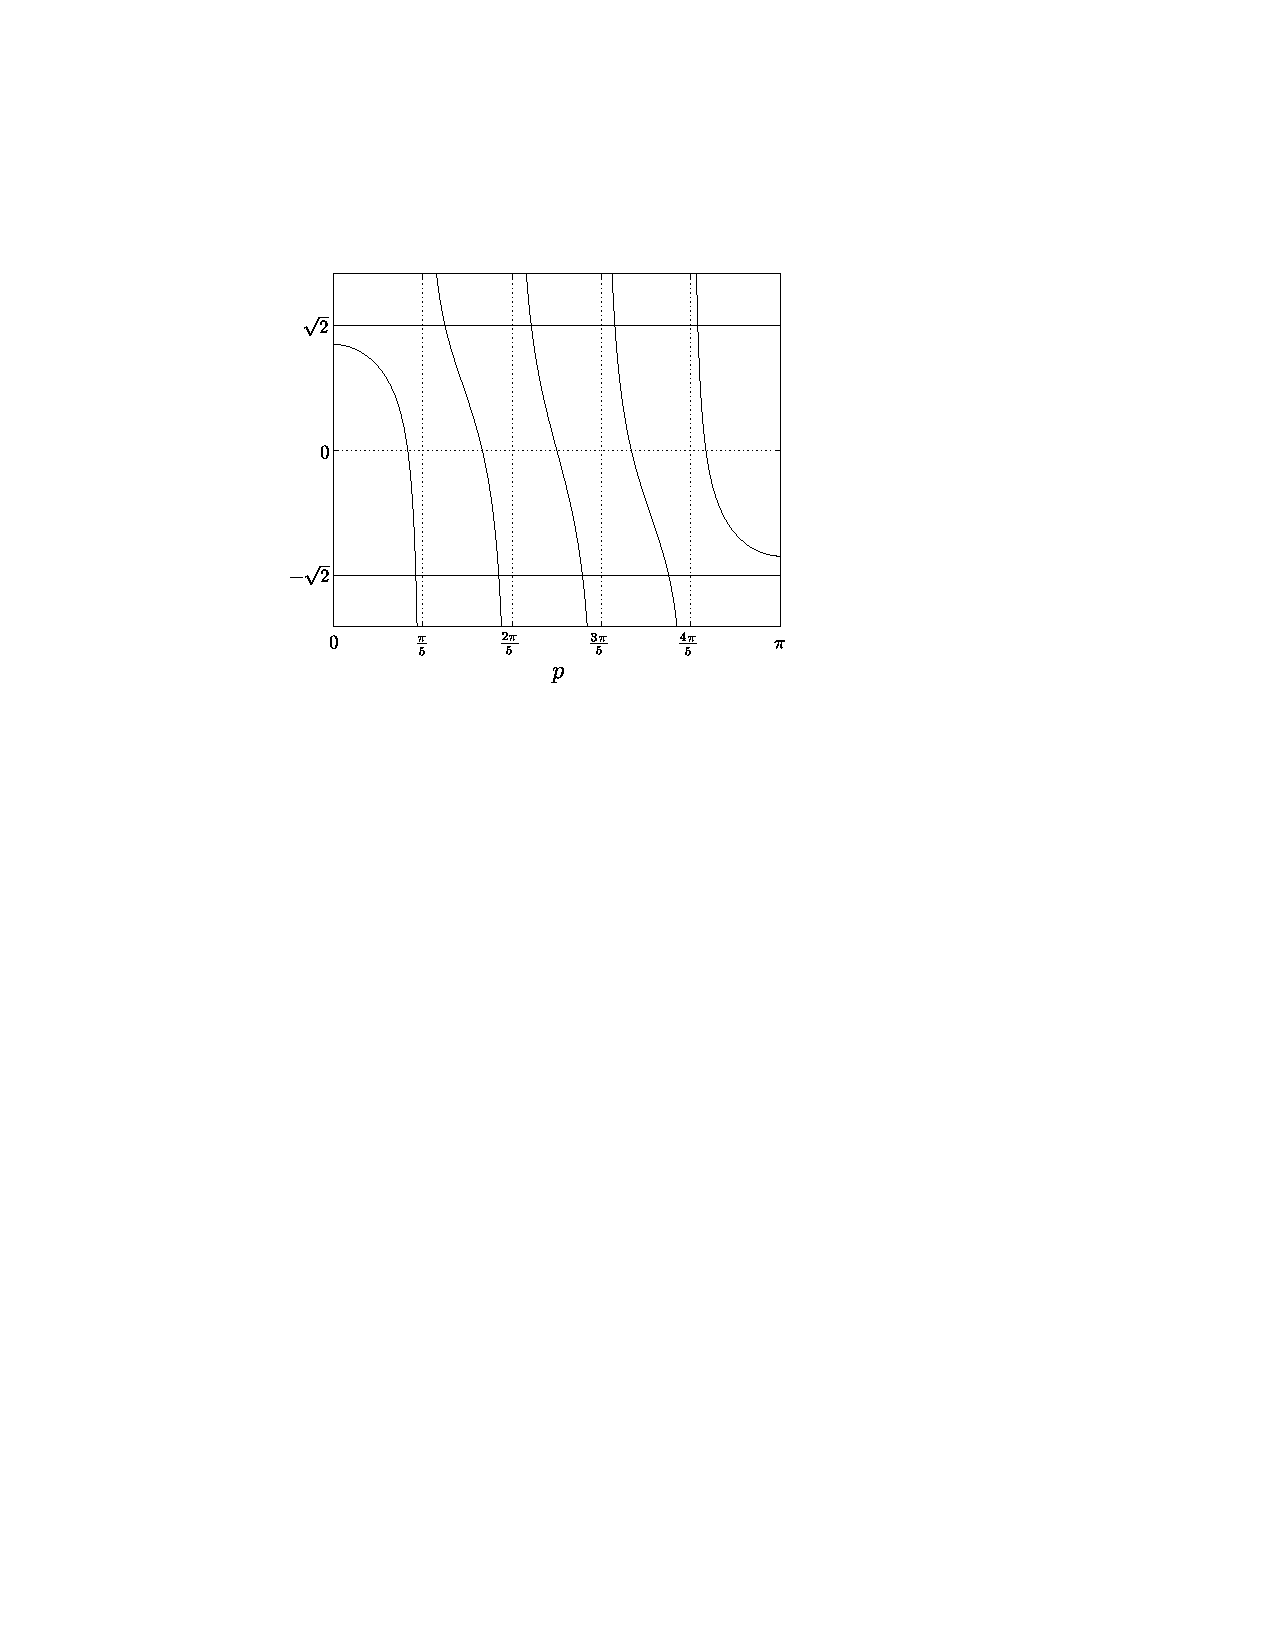
\includegraphics[width=0.7\textwidth]{cons.png}
\caption{Left hand side of (\ref{eq:constraint}) for $n=5$.}
\label{fig:constraint}
\end{figure}

\end{proof sketch}


\subsection{An efficient quantum algorithm for traversing $G^{\prime}_n$}
To summarize, with theorem \ref{thm:hitting}, we an efficient quantum algorithm for traversing $G^{\prime}_n$. The computer is prepared in the state corresponding to the $\ent$, and the quantum walk is simulated using the construction described in Section \ref{subsec:implement}.  After
running the walk for an appropriate $t=\poly(n)$, the state of the computer is
measured. The probability of finding the name of the $\exit$ can be $O(1/n)$.  By
repeating this process $\poly(n)$ times, the success probability can be
made arbitrarily close to 1. 



%%%%%%%%%%%%%%%%%%%%%%%%%%%%%%%%%%%%%%%%%%%%%%%%%%%%%%%%%%%%%%%%%%%%%%%%%%%%%%%

\section{Classical lower bound}\label{sec:lowerbound}

Now we want to proof that no classical algorithm can find the $\exit$ with high
probability in subexponential time. The authors achieve this by a sequence of games that the first game is equivelant to the original traversal problem, and each subsequent game is essentially as easy to win. Finally, they will show that the easiest game cannot be won in subexponential time.

\subsection{Turn the original problem to a game}

\begin{game}\label{game:original}
  The oracle contains a random set of names for the vertices of the
  randomly chosen graph $G_n'$ such that each vertex has a distinct
  $2n$-bit string as its name and the $\ent$ vertex has the name $0$.  In
  addition, the edges of the graph are randomly colored as described
  above.
%
  At each step, the algorithm sends a $2n$-bit string to the oracle, and
  if there exists a vertex with that name, the oracle returns the names of
  the neighbors of that vertex and the colors of the edges that join
  them.
%
  The algorithm wins if it ever sends the oracle the name of the $\exit$
  vertex.
\end{game}

\subsection{Restriction to known vertices}


\begin{game}\label{game:tree}
  The oracle contains a graph, set of vertex names, and edge coloring as
  described in Game \ref{game:original}.
%
  At each step, the algorithm sends the oracle the name of the $\ent$
  vertex or the name of a vertex it has previously been sent by the
  oracle.  The oracle then returns the names of the neighbors of that
  vertex and the colors of the edges that join them.
%
  The algorithm wins it ever sends the oracle the name of the $\exit$
  vertex.
\end{game}

The win rate of the game is lower, but bounded with exponentially small term. This is because the chance that the original game algorithm can discover the name of a vertex that it is not told by the oracle is at most $t (2^{n+2}-2) / 2^{2n}$, and unless this happens, the algorithms will have similar behavior.

\subsection{Removal of coloring}

The authors make a consistent coloring that does not provide information for any classical quantum algorithm. At each vertex in an even numbered column, randomly color the incident edges $A,B,C$.  At each vertex in an odd numbered column, randomly append $1,2,3$ to the colors of the incident edges.  The edges are then colored with one of nine colors, $A1,A2,A3,B1,\ldots,C3$.  Because of the structure of $G_n'$, any such coloring is consistent. Also, since the parity of columns is the only information required for a classical algorithm to make up the color of an edge, and this information is always available to an algorithm that can only traverse a connected subgraph, the coloring cannot provide more information to the algorithms.

\begin{game}\label{game:nocolors}
  The oracle contains a graph and a set of vertex names as described in
  Game \ref{game:original}.
%
  At each step, the algorithm sends the oracle the name of the $\ent$
  vertex or the name of a vertex it has previously been sent by the
  oracle.  The oracle then returns the names of the neighbors of that
  vertex.
%
  The algorithm wins it ever sends the oracle the name of the $\exit$
  vertex.
\end{game}

\subsection{Adding a new win condition ---  Finding a Cycle}

\begin{game}\label{game:nocycles}
  The oracle contains a graph and a set of vertex names as described in
  Game \ref{game:original}.
%
  At each step, the algorithm and the oracle interact as in Game
  \ref{game:nocolors}.
%
  The algorithm wins it ever sends the oracle the name of the $\exit$
  vertex, or if the subgraph it has seen contains a cycle.
\end{game}

Game \ref{game:nocycles} is clearly easier to win than Game \ref{game:nocolors}. And by this, we restrict the subgraph an algorithm sees must be a rooted binary tree

\subsection{Reformulation as Tree Embedding}

For a rooted binary tree $T$, we define an embedding of $T$ into $G$ to be a function $\pi$ from the vertices of $T$ to the vertices of $G$ such that $\pi(\root) = \ent$ and for all vertices $u$ and $v$ that are neighbors in $T$, $\pi(u)$ and $\pi(v)$ are neighbors in $G$.  We say that an embedding of $T$ is {\em proper} if $\pi(u) \not = \pi(v)$ for $u \ne v$.  We say that a tree $T$ {\em exits} under an embedding $\pi$ if $\pi(v) = \exit$ for some $v \in T$.

 A random embedding of a tree is obtained by setting $\pi(\root) = \ent$ and then mapping the rest of $T$ into $G$ at random recursively.


\begin{game}\label{game:randomembedding}
  The algorithm outputs a rooted binary tree $T$ with $t$ vertices in
  which each internal vertex has two children.  A random embedding $\pi$ is chosen.
  The algorithm wins if $\pi$ is an improper embedding of $T$ in $G_n'$ or if $T$ exits $G_n'$ under $\pi$.
\end{game}


\begin{lemma}\label{lem:equivalence}
For any algorithm $A$ for Game \ref{game:nocycles} that uses at most $t$
queries of the oracle, there exists an algorithm $A'$ for Game
\ref{game:randomembedding} that outputs a tree of at most $t$ vertices
such that for all graphs $G$,
\be
    \mathbb{P}^{G}_{\ref{game:nocycles}}(A) 
  = \mathbb{P}^{G}_{\ref{game:randomembedding}}(A')
\,.
\ee
\end{lemma}

\begin{proof}
Algorithm $A$ halts if it ever finds a cycle, exits, or uses $t$ steps.
Algorithm $A'$ will generate a (random) tree by simulating $A$.  Suppose
that vertex $a$ in graph $G$ corresponds to vertex $a'$ in the tree that
$A'$ is generating.  If $A$ asks the oracle for the names of the neighbors
of $a$, $A'$ generates two unused names $b'$ and $c'$ at random and uses
them as the neighbors of $a'$.  Now $b'$ and $c'$ correspond to $b$ and
$c$, the neighbors of $a$ in $G$.  Using the tree generated by $A'$ in
Game \ref{game:randomembedding} has the same behavior as using $A$ in Game
\ref{game:nocycles}.
\end{proof}

\noindent
Finally, we bound the probability that an algorithm wins Game \ref{game:randomembedding}:

\begin{lemma}\label{lem:ourGraphs}
For rooted trees $T$ of at most $2^{n/6}$ vertices,
\be
 \max_{T}
  \expec{G}{\mathbb{P}^G(T)}
  \leq 3 \cdot 2^{-n/6}.
\ee
\end{lemma}

\begin{proof sketch}

\begin{enumerate}
    \item Define $\frac{n}{2}$-subtrees
    \item Show it is hard to reach roots of $\frac{n}{2}$-subtrees on the right side
    \item Show it is hard to form a cycle by considering the lists of subtrees passed corresponding to the paths in the tree $T$ that forms a cycle.
\end{enumerate}

Part 3 is the core of this paper, one can find the full statement in the original paper \cite{EXP03}. It is the place that the difference between $G_n$ and $G^{\prime}_n$ is used.

\end{proof sketch}

With the above results, we can have the final theorem.

\begin{theorem}
Any classical algorithm that makes at most $2^{n/6}$ queries to the oracle
finds the $\exit$ with probability at most $4 \cdot 2^{-n/6}$.
\end{theorem}


%%%%%%%%%%%%%%%%%%%%%%%%%%%%%%%%%%%%%%%%%%%%%%%%%%%%%%%%%%%%%%%%%%%%%%%%%%%%%%%
\section{Conclusion}\label{sec:conclusion}

\begin{itemize}
    \item The authors show that $\BQP^{A} \neq \BPP^{A}$ for the oracle $A=U$ corresponding to graph $G^{\prime}_n$.
    \item The separation is exponential and is not achieved by Fourier based method but with pure quantum inference effect.
\end{itemize}

\section{Discussion and Open Problems}\label{sec:discussion}

\begin{itemize}
    \item The results can also be cast in terms of a graph reachability problem (a decision problem).
    \item The relation of complexity classes relative to oracles provides intuitions and insights to the relation of original classes, but it cannot be used to show the relation itself. (Relativization \cite{MITACT16}) So it remains a challenge to determine $\BQP \overset{?}= \BPP$.
    \item Can one find more other techniques for implementing quantum walks?
    \item Are there interesting problems that are considered classically hard can be solve efficiently with quantum walks?
        \begin{itemize}
            \item To my knowledge, there is a machine-learning work aiming to predict speedup by quantum walk\cite{ALEX19}.
            \item Can we give explicit characteristics (sufficient and necessary conditions)?
        \end{itemize}
\end{itemize}



%%%%%%%%%%%%%%%%%%%%%%%%%%%%%%%%%%%%%%%%%%%%%%%%%%%%%%%%%%%%%%%%%%%%%%%%%%%%%%%
% References

\begin{thebibliography}{9}
\bibitem{Sim94}
  D. Simon,
  {\em On the power of quantum computation},
  Proc. 35th IEEE Symposium on the Foundations of Computer Science,
  116 (1994).
\bibitem{FG98}
  E. Farhi and S. Gutmann,
  {\em Quantum computation and decision trees},
  Phys. Rev. A {\bf 58}, 915 (1998).
\bibitem{MITACT16}
  Dana Moshkovitz,
  {\em Advanced Complexity Theory Lecture 2: Relativization}, \\
  https://ocw.mit.edu/courses/mathematics/18-405j-advanced-complexity-theory-spring-2016/lecture-notes/MIT18/\_405JS16\_Relativ.pdf.
\bibitem{EXP03}
    Childs, Andrew M., et al,
    {\em Exponential algorithmic speedup by a quantum walk},
    Proceedings of the thirty-fifth annual ACM symposium on Theory of computing. 2003.
\bibitem{NC00}
  M. A. Nielsen and I. L. Chuang,
  {\em Quantum Computation and Quantum Information},
  (Cambridge University Press, Cambridge, 2000).
 \bibitem{ALEX19}
 Melnikov, Alexey A., Leonid E. Fedichkin, and Alexander Alodjants,
 {\em Predicting quantum advantage by quantum walk with convolutional neural networks},
 New Journal of Physics 21.12 (2019): 125002.
  
\end{thebibliography}

\end{document}

